% Template for PLoS
% Version 3.1 February 2015
%
% To compile to pdf, run:
% latex plos.template
% bibtex plos.template
% latex plos.template
% latex plos.template
% dvipdf plos.template
%
% % % % % % % % % % % % % % % % % % % % % %
%
% -- IMPORTANT NOTE
%
% This template contains comments intended 
% to minimize problems and delays during our production 
% process. Please follow the template in                structions
% whenever possible.
%
% % % % % % % % % % % % % % % % % % % % % % % 
%
% Once your paper is accepted for publication, 
% PLEASE REMOVE ALL TRACKED CHANGES in this file and leave only
% the final text of your manuscript.
%
% There are no restrictions on package use within the LaTeX files except that 
% no packages listed in the template may be deleted.
%
% Please do not include colors or graphics in the text.
%
% Please do not create a heading level below \subsection. For 3rd level headings, use \paragraph{}.
%
% % % % % % % % % % % % % % % % % % % % % % %
%
% -- FIGURES AND TABLES
%
% Please include tables/figure captions directly after the paragraph where they are first cited in the text.
%
% DO NOT INCLUDE GRAPHICS IN YOUR MANUSCRIPT
% - Figures should be uploaded separately from your manuscript file. 
% - Figures generated using LaTeX should be extracted and removed from the PDF before submission. 
% - Figures containing multiple panels/subfigures must be combined into one image file before submission.
% For figure citations, please use "Fig." instead of "Figure".
% See http://www.plosone.org/static/figureGuidelines for PLOS figure guidelines.
%
% Tables should be cell-based and may not contain:
% - tabs/spacing/line breaks within cells to alter layout or alignment
% - vertically-merged cells (no tabular environments within tabular environments, do not use \multirow)
% - colors, shading, or graphic objects
% See http://www.plosone.org/static/figureGuidelines#tables for table guidelines.
%
% For tables that exceed the width of the text column, use the adjustwidth environment as illustrated in the example table in text below.
%
% % % % % % % % % % % % % % % % % % % % % % % %
%
% -- EQUATIONS, MATH SYMBOLS, SUBSCRIPTS, AND SUPERSCRIPTS
%
% IMPORTANT
% Below are a few tips to help format your equations and other special characters according to our specifications. For more tips to help reduce the possibility of formatting errors during conversion, please see our LaTeX guidelines at http://www.plosone.org/static/latexGuidelines
%
% Please be sure to include all portions of an equation in the math environment.
%
% Do not include text that is not math in the math environment. For example, CO2 will be CO\textsubscript{2}.
%
% Please add line breaks to long display equations when possible in order to fit size of the column. 
%
% For inline equations, please do not include punctuation (commas, etc) within the math environment unless this is part of the equation.
%
% % % % % % % % % % % % % % % % % % % % % % % % 
%
% Please contact latex@plos.org with any questions.
%
% % % % % % % % % % % % % % % % % % % % % % % %

\documentclass[10pt,letterpaper]{article}
\usepackage[top=0.85in,left=2.75in,footskip=0.75in]{geometry}

% Use adjustwidth environment to exceed column width (see example table in text)
\usepackage{changepage}

% Use Unicode characters when possible
\usepackage[utf8]{inputenc}

% textcomp package and marvosym package for additional characters
\usepackage{textcomp,marvosym}

% fixltx2e package for \textsubscript
\usepackage{fixltx2e}

% amsmath and amssymb packages, useful for mathematical formulas and symbols
\usepackage{amsmath,amssymb}

% cite package, to clean up citations in the main text. Do not remove.
\usepackage{cite}

% Use nameref to cite supporting information files (see Supporting Information section for more info)
\usepackage{nameref,hyperref}

% line numbers
\usepackage[right]{lineno}

% ligatures disabled
\usepackage{microtype}
\DisableLigatures[f]{encoding = *, family = * }

% rotating package for sideways tables
\usepackage{rotating}

% Remove comment for double spacing
%\usepackage{setspace} 
%\doublespacing

% Text layout
\raggedright
\setlength{\parindent}{0.5cm}
\textwidth 5.25in 
\textheight 8.75in

% Add more colors for editting
\usepackage[usenames,dvipsnames]{xcolor}

% Bold the 'Figure #' in the caption and separate it from the title/caption with a period
% Captions will be left justified
\usepackage[aboveskip=1pt,labelfont=bf,labelsep=period,justification=raggedright,singlelinecheck=off]{caption}

% Use the PLoS provided BiBTeX style
\bibliographystyle{plos2015}

% Remove brackets from numbering in List of References
\makeatletter
\renewcommand{\@biblabel}[1]{\quad#1.}
\makeatother

% Leave date blank
\date{}

% Header and Footer with logo
\usepackage{lastpage,fancyhdr,graphicx}
\usepackage{epstopdf}
\pagestyle{myheadings}
\pagestyle{fancy}
\fancyhf{}
\rfoot{\thepage/\pageref{LastPage}}
\renewcommand{\footrule}{\hrule height 2pt \vspace{2mm}}
\fancyheadoffset[L]{2.25in}
\fancyfootoffset[L]{2.25in}
\lfoot{\sf PLOS}

%% Include all macros below

\newcommand{\lorem}{{\bf LOREM}}
\newcommand{\ipsum}{{\bf IPSUM}}
\newcommand{\citex}{\textcolor{red}{\textbf{CITE}} }
\newcommand{\X}{\textcolor{red}{\textbf{X}} }
\usepackage[colorinlistoftodos]{todonotes} % comments in margins
\reversemarginpar
\setlength{\marginparwidth}{5cm}
\definecolor{flame}{rgb}{0.89, 0.35, 0.13}
\newcommand{\jri}[1]{\todo[size=\scriptsize, color=SkyBlue]{#1}}
\newcommand{\pb}[1]{\todo[size=\scriptsize, color=Bittersweet]{#1}} %too perfect.


%% END MACROS SECTION


\begin{document}
\vspace*{0.35in}

% Title must be 250 characters or less.
% Please capitalize all terms in the title except conjunctions, prepositions, and articles.
\begin{flushleft}
{\Large
\textbf\newline{ Bioinformatic analyses of genomic composition of tandem repeats in grasses %Applications and Limiations of De-Novo Centromeric Repeat Assembly in Grasses
}
}
\newline
% Insert author names, affiliations and corresponding author email (do not include titles, positions, or degrees).
\\
Paul Bilinski*\textsuperscript{1}%\Yinyang},
Jiming Postdoc/student\textsuperscript{2,},
Anne Lorant\textsuperscript{1},
Matthew B. Hufford\textsuperscript{3,},
Jiming Jiang\textsuperscript{2,},
Jeffrey Ross-Ibarra*\textsuperscript{1,4}
%Name3 Surname\textsuperscript{2,\textcurrency a},
%Name4 Surname\textsuperscript{2,\ddag},
%Name5 Surname\textsuperscript{2,\ddag},
%Name6 Surname\textsuperscript{2},
%Name7 Surname\textsuperscript{3,*},
%with the Lorem Ipsum Consortium\textsuperscript{\textpilcrow}
\\
\bigskip
\bf{1} Dept. of Plant Sciences, University of California, Davis, CA, USA
\\
\bf{2} Dept. of Horticulture, University of Wisconsin-Madison, Madison, WI USA
\\
\bf{3} Department of Ecology, Evolution, and Organismal Biology, Iowa State University, Ames, Iowa, USA
\\
\bf{4} Center for Population Biology and Genome Center, University of California, Davis, CA, USA
\\
\bigskip

% Insert additional author notes using the symbols described below. Insert symbol callouts after author names as necessary.
% 
% Remove or comment out the author notes below if they aren't used.
%
% Primary Equal Contribution Note
%\Yinyang These authors contributed equally to this work.

% Additional Equal Contribution Note
% Also use this double-dagger symbol for special authorship notes, such as senior authorship.
%\ddag These authors also contributed equally to this work.

% Current address notes
%\textcurrency a Insert current address of first author with an address update
% \textcurrency b Insert current address of second author with an address update
% \textcurrency c Insert current address of third author with an address update

% Deceased author note
%\dag Deceased

% Group/Consortium Author Note
%\textpilcrow Membership list can be found in the Acknowledgments section.

% Use the asterisk to denote corresponding authorship and provide email address in note below.
* pbilinski@ucdavis.edu, rossibarra@ucdavis.edu

\end{flushleft}
% Please keep the abstract below 300 words
\section*{Abstract}
\jri{JRI comments}
\pb{PB comments}
In studying genomic architecture, highly repetitive regions have historically posed a challenge when investigating sequence variation and content.
High-throughput sequencing has enabled researchers to use whole-genome shotgun sequencing to estimate the abundance of repetitive sequence, and these methodologies have been recently applied to centromeres.
Here, we utilize sequence assembly and read mapping to identify and quantify the genomic abundance of different tandem repeat sequences.
Previous research has posited that the highest abundance tandem repeat in eukaryotic genomes is often the centromeric repeat, and we pair our bioinformatic pipeline with fluorescent in-situ hybridization data to test this hypothesis.
We find that de novo assembly and bioinformatic filters can successfully identify repeats with homology to known tandem repeats.
Fluorescent in-situ hybridization, however, shows that de novo assembly fails to identify novel centromeric repeats, instead identifying other potentially important repetitive sequences.
Together, our results test the applicability and limitations of using de novo repeat assembly of tandem repeats to identify novel centromeric repeats.
Building on our findings of genomic composition, we also set forth a method for exploring the repetitive regions of non-model genomes whose diversity limits the applicability of established genetic resources.

% Please keep the Author Summary between 150 and 200 words
% Use first person. PLOS ONE authors please skip this step. 
% Author Summary not valid for PLOS ONE submissions.   
\section*{Author Summary}
%ROUGH: Melters et al say they can use most abundant tandem repeat to get centromeric repeat.
%we build a similar pipeline, identify most common tandem repeat, filter against known repeats, and identify the cent repeat in known genomes
%in several grasses we find novel repeats, and use fish to show that these are likely NOT cent repeats
%however, our pipeline also identifies a possible knob repeat in a nepalensis, whose sequence diversity is entirely new and potentially ancestral to many grasses.
%data: 
%bunch of grasses from across andropogonae (Matt as author)
%sequence them (Anne as author)
%identify canonical cent repeat (paul)
%FISH for repeat in known and unknown (jiming udig and hypdip)
%potentially FISH for the knob like repeat (ask Jiming to follow it up?)

\linenumbers

\section*{Introduction}

Sequencing technologies have facilitated genome assembly for many non-model organisms, bringing a tremendous amount of data to the field of comparative genomics.
Unfortunately, this data has an overrepresentation of genic regions as short read data currently struggles to accurately assemble repetitive regions.
Though repetitive DNA was once disregarded as "junk DNA", research continues to unravel the many functions of repetitive DNA, spurring a growing interest in a better understanding of the evolutionary history and genomic composition of repeats.
Plants are known for their high repetitive content and serve as an excellent model in which to investigate questions regarding repeat sequence evolution.
Plant genomes can be up to 85\% repetitive \cite{Schnable2009}.
The repetitive sequence found in plants can be classified into two broad categories, either dispersed around the genome because the repeat is derived from transposable elements (TEs) or tandemly repeated sequence.
TE derived repeats comprise the majority of many eukaryotic genomes and are recognized for their different modes of amplification, being divided into class I (RNA intermediate) or class II (DNA intermediate).
TEs have been shown to impact gene expression \cite{waterland2003transposable} and chromatin status \cite{miura2001mobilization}, functions which can have strong impacts on overall phenotype.
The field of comparative genomics has shed light on the evolutionary history of TEs through the phylogeny \cite{rokas2000rare}, informed hypotheses about TE expansion and contraction \cite{hawkins2008repeated}, and traced TE function in related organisms \cite{daniels1990evidence}.\pb{JRIHELP i think the citations are correct, but please verify that rokas and daniels are the most appropriate citations}

In comparison to the wealth of TE data across organisms, little is known about the function and evolutionary history of tandem repeats.
Tandem repeats comprise a smaller percentage of the genome, though that percentage composition can vary wildly across different phylogenetic groups \cite{gaut2008selection}.
The most common tandem repeats are found in the gene poor but structurally important telomeres and centromeres.
Both telomeres and centromeres are highly heterochromatic, however, the mechanisms by which tandem repeat sequences contribute to the formation of centromeres or telomeres are only vaguely known.
Previous research has also shown that tandem repeats are not necessary for the formation of centromeres \cite{zhong2002centromeric}, suggesting that tandem repeats may serve as a placeholder for an epigenetic signal that governs heterochromatin formation.
Tandem repeats are also found in other types of heterochromatin that suppress local recombination such as knobs in the model organism maize (\emph{Zea mays}, \cite{chang1974interaction}).

In an effort to better understand tandemly repeated sequence, researchers have begun to develop new methodologies that can study sequence variation of repeats.
Studies that have paired chromatin immuniprecipitation (ChIP) for centromere proteins with bioinformatic identification of repetitive sequence have proven successful in identifying centromere repeats \cite{gong2012repeatless}.
However, ChIP is labor intensive and difficult to perform in a high-throughput manner, leading other studies to utilize only bioinformatics and whole genome short read data to identify centromere repeats.
Tapping into the plethora of previously published sequence data, Melters et al \cite{melters2013comparative} pair shotgun short read sequencing from different organisms with de novo repeat assembly, effectively constructing a series of consensus sequences of tandem repeats genome wide.
They applied their approach broadly across more than 280 plant and animal taxa, relying on model organisms to serve as positive controls.
They assume that the most abundant tandem repeat in all taxa is the centromere repeat, and use this assumption to study centromere repeat evolution broadly.
While the approach appears to work well for animals, earlier work suggests that this assumption may not apply broadly to plants.
Using a similar pipeline applied to 454 shotgun reads in \emph{Solanum} species, Torres et al identified telomeric repeats as the highest frequency kmer \cite{torres2011organization}, and heterochromatic knobs in maize also obstruct the identification of the centromere repeat \cite{dennis1984knob}. \pb{not sure what to cite here, so just went with the already cited knob paper.  Is this appropriate?}

In our study, we aim to apply the basic pipeline of tandem repeat consensus assembly to a narrower phylogenetic group within the grasses to better understand tandem repeat contribution to genomic composition.
We select species from across the tribe andropogoneae, including the agriculturally important species maize and sorghum.
Maize and sorghum are ideal anchor species as both have reference genomes and their centromere repeats are diverged from one another \cite{paterson2009sorghum,Schnable2009}, allowing us to also test the Melters et al \cite{melters2013comparative} hypothesis regarding centromere repeat sequence and it's genomic abundance.
Because previous work has shown that sequencing libraries prepared through identical methods retain relative composition of repetitive content \cite{bilinski2014diversity},\jri{wha? i don't think anyone has shown this. instead they've shown the converse}\pb{JRIHELP if this doesnt apply, then isnt my entire phd a farce?  identical library prep keeps relative repeat content across samples.} we elect to re-sequence species used in the study.
We examine sequence similarity and genomic composition of highly abundant tandem repeats across the phylogeny, determine their homology to known centromere repeats, and perform fluorescent in-situ hybridization to test whether novel high abundance repeats show patterns consistent with other centromere repeats.
We show that the assumption of Melters et al. \cite{melters2013comparative} that the highest abundance tandem repeat is a centromere is not supported in grasses, especially when the centromere repeat is novel or unknown.
However, we show that de novo tandem repeat assembly can be used to identify entirely novel repeats such as the knob-like repeat in \emph{Arundinella}.
The ability to identify novel repeats from low cost sequencing can enable a new type of comparative genomic study that tracks the evolution of genomic composition.\jri{not sure I buy this.your paper suggests method don't work well!}\pb{it shows you cant assume its a centromere repeat, but you can still track abundance of tandem repeats generally in the genome}

% You may title this section "Methods" or "Models". 
% "Models" is not a valid title for PLoS ONE authors. However, PLoS ONE
% authors may use "Analysis" 
\section*{Materials and Methods}

\subsection*{Sequencing}
DNA was isolated from leaf tissue using the DNeasy plant extraction kit (Qiagen) according to the manufacturer’s instructions. 
The samples were quantified using Qubit (Life Technologies) 1ug of DNA was fragmented using the bioruptor (Diagenode) with cycles of 30 seconds on, 30 seconds off. 
The DNA fragments were prepared for Illumina sequencing. 
First, DNA fragments were repaired with the End-Repair enzyme mix (New England Biolab). 
A deoxyadenosine triphosphate was added at each 3'ends with the Klenow fragment (New England Biolab). 
Illumina Trueseq adapters (Affymetrix) were added with the Quick ligase kit (New England Biolab). 
Between each enzymatic step, cDNA was washed with sera-mags speed beads(Fisher Scientific).
Samples were multiplexed and sequenced in one lane of Miseq (UC Davis Genome Center Sequencing Facility) for 150 paired-end base reads with an insert size of approximately 350 bases.
Parsing of reads was performed with in house scripts, and forward reads were used for all analyses.

\subsection*{Phylogenetic Tree Reconstruction}
We downloaded sequence data for two inter-genic spacers and one chloroplast gene at NCBI (sequences available on \url{https://github.com/paulbilinski/Github_centrepeat}).
Sequences were aligned using seven iterations of MUSCLE \cite{edgar2004muscle}, and concatenated in order to build a neighbor joining tree using Jukes-Cantor distance.
The topologies represent approximate relationships that have been discussed in greater detail in several studies  \cite{wu2012phylogeny,skendzic2007phylogenetics}.
The topology varies slighty between studies, as some nodes are collapsed into polytomies.\jri{do they agree? is wu 2012 part of wu-tang?}\pb{nothing in phylogenetics ever agrees and includes all of our exact species.  thats why i went to make my own. also, wu-tang clan aint nothing to trifle with.}

\begin{figure}[h]
\begin{center}
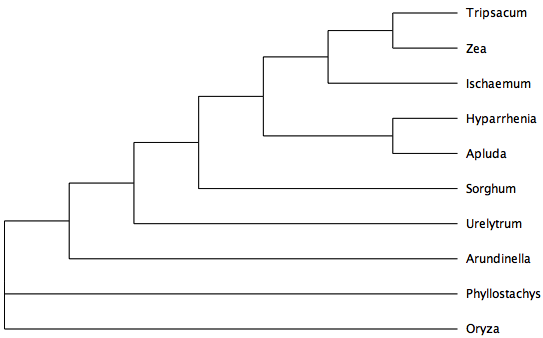
\includegraphics[width=4in]{Phylotree_centrepeat.png}
\end{center}
\caption{{\bf Neighbor joining tree of evolutionary relationships between the grasses studied.}
Topology is an approximate cladogram, reconstructed from 3 neutrally evolving loci.
A more detailed discussion of possible relationships is available in \cite{wu2012phylogeny,skendzic2007phylogenetics}.  
\emph{Oryza} and \emph{Phyllostachys} are both outside the andropogoneae tribe.}
\label{phylotree}
\end{figure}
\jri{is that a cladogram or an NJ tree?}\pb{NJ tree is a type of cladogram, but if you prefer NJ tree name then so it is}
\subsection*{Assembly and Genomic Composition of Centromere Repeats}

% For figure citations, please use "Fig." instead of "Figure".

We used MIRA (Chevreux et al. 1999, version 4.0; job = genome,denovo,accurate, parameters = -highlyrepetitive -NW:cnfs=no -NW:mrnl=200 -HS:mnr=no)to assemble low coverage libraries.
We ran Tandem Repeat Finder \cite{benson1999tandem}  (TRF) on all assembled contigs to select only those that contained tandem repeats. 
Parameters for TRF were Match = 2, Mismatch = 7, Indel = 7, Probability of match = 80, Probability of indel = 10, Min score = 50, and Max period = 2000.
%Previous surveys across both plant and animal taxa show that centromere repeats are short and often the most abundant tandem repeat \cite{melters2013comparative}.  
%However, studies have shown that in certain grasses such as \emph{Zea mays} the centromere repeat is not the most abundant tandem repeat due to the presence of knobs (Not sure what to cite).
%To ensure that we were selecting the most abundant tandem repeat with no homology to known knob repeats, we identified assembled contigs with homology to known knob repeats via blastn and removed them.
%Those non-knob-like tandem repeat assemblies for each species were then used as a mapping reference for Mosaik, which stores information about multiply mapping reads (version 1.0; parameters optimized for tandem repetitive elements as in \cite{bilinski2014diversity}.
To discover the genomic composition of each tandemly repeated contig, we used Mosaik \cite{lee2014mosaik}, which stores information about multiply mapping reads (version 1.0; parameters optimized for tandem repetitive elements as in \cite{bilinski2014diversity}.
Low coverage libraries were mapped against the reference and contigs were ranked by the number of reads aligning to each contig.
The top ranking contig was extracted, and the number of reads aligning to it was recorded from the assembly ace files.
We then blasted (-evalue 1E-1 -outfmt 7 -max\_target\_seqs 15000 -task blastn) the top ranking contig against all other TRF assemblies, removed assemblies with BLAST homology.
This process was repeated 4 times to identify the genomic composition of the 4 highest abundance tandem repeat groups. 
Scripts and step by step guides are available on \url{https://github.com/paulbilinski/Github_centrepeat}.
%If the highest abundance contig shared homology with a known non-centromeric repeat in grasses, it was discarded.  
%From the highest abundance polymer and our TRF identifications, we extracted the single chimeric monomer produced from TRF.  
%We blasted the monomer against all other TRF assemblies, and used the monomer (narrow) and list of polymers with homology to the monomer (broad) as mapping references to identify genomic abundance of the putative centromere repeat.


\begin{figure}[h]
\begin{center}
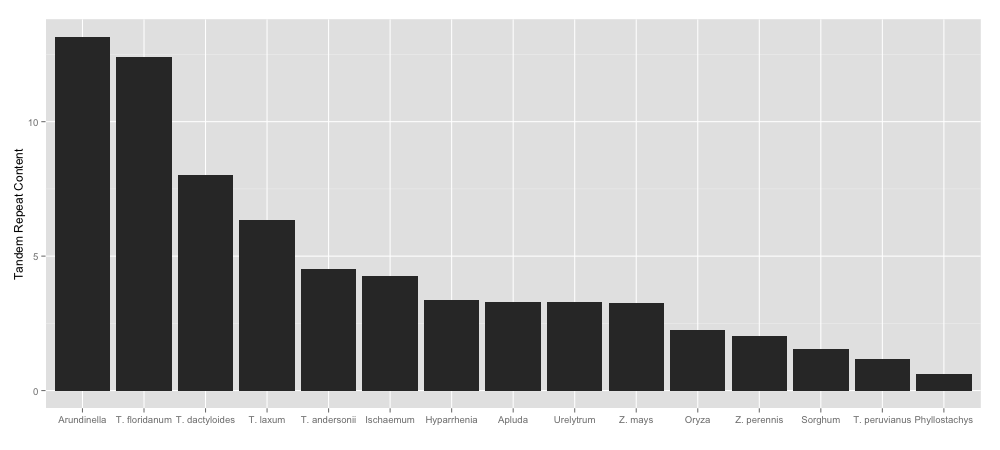
\includegraphics[width=4in]{total_trf.png}
\end{center}
\caption{{\bf Percentage genomic composition of all tandem repeat contigs in monocot taxa.}
Values are derived from the sum of all reads mapping to any tandemly repetitive contig derived from TRF after MIRA assembly.  
Species are ordered from highest to lowest percentage tandem repeat content.}
\label{totaltrf}
\end{figure}

\subsection*{Fluorescent In-Situ Hybridization}
Sequences for FISH probes had (Udig 96\% identity; Hyp 96\% identity) as they were consensus sequences from TRF assemblies of highly similar high abundance contigs.
[Text from Jiming here].
Probes used should be included in here or the supplement.


% Results and Discussion can be combined.
\section*{Results}
Assembly of low coverage whole genome shotgun Illumina data produced several thousand contigs in each species from our panel.
From these, TRF was able to identify between 300 and 15,000 contigs comprised of tandem repeats in each taxa.
The number of contigs made of tandem repeats varied between taxa based on coverage and overall genomic repetitive content.
We mapped whole genome shotgun Illumina data against all post-TRF contigs to approximate genomic composition of all tandemly repetitive sequence in our panel \ref{totaltrf}.
Mapping against all contigs enables us to capture the broad diversity of all tandem repeats.
Results show that our taxa vary greatly in their total tandem repeat content, ranging from over 13\% to under 1\%.
We see high tandem repeat content within the \emph{Tripsacum} and \emph{Arundinella} genera, though \emph{Tripsacum} taxa show large variations.
We wanted to see whether total tandem repeat content correlated with genome size.
Using the Kew C-Value database \cite{kewc}, we obtained point estimates for genome size in each of our taxa.
The correlation between total tandem repeat content and genome size was poor (r=0.05).

We further wanted to investigate the proportional contribution of the most common tandem repeat classes in each of our taxa.
To do so, we ranked the mapping abundance of all post-TRF contigs.
We used the number of reads mapping to the top ranked contig as its abundance, and removed any similar contigs from our rankings using BLAST homology (See methods for parameters).
We repeated this for the top four tandem repeats in each genome.
Results showed that most taxa had one tandem repeat class at much higher abundance than other tandem repeats.
In all taxa except for \emph{Arundinella}, only the top contig exceeded 1\% of genomic composition.
\emph{Sorghum}, \emph{Phyllostchys}, \emph{Ischaemum}, and \emph{Apluda} showed the largest difference between the top ranked contig and the second ranked contig.
In the sister genera \emph{Zea} and \emph{Tripsacum}, while the top ranked contig showed immense variation, the second ranked contig had a relatively constant abundance near half a percent.
The \emph{Arundinella} genome seems unique in that it has several high abundance different class tandem repeats.

In our analysis of genomic contribution from each class of tandem repeat, we found that most genomes had one class of tandem repeat far above the rest.
Previous works have posited that this repeat is the centromeric repeat in many species \cite{melters2013comparative}.
We wanted test this hypothesis in taxa with known centromere repeats as well as in taxa with uncharacterized genomes.
For \emph{Oryza} and \emph{Sorghum}, whose centromere repeats are known, the assumption that the highest abundance tandem repeat is the centromere repeat held true in our analyses.
In \emph{Zea} and \emph{Tripsacum}, where knob repeats are known to exist \cite{dennis1984knob}, the centromere repeat is not the highest abundance tandem repeat, though it is ranked within the top four.
\emph{Apluda}'s top ranked contig shared homology and a common monomer repeat length with the 137bp \emph{Sorghum} centromere repeat, suggesting that the method is robust in \emph{Apluda} as well.
\emph{Ischaemum}'s monomer was also 137bp long, but only shared slight homology to \emph{Sorghum}.
However, our analyses also yielded several taxa whose top ranked contig had no homology to known centromere repeats.
We chose to test the robustness of the Melters et al \cite{melters2013comparative} assumption in these taxa with fluorescent in-situ hybridization (FISH).
FISH from the de novo constructed repeat of \emph{Urelytrum} showed a strong spatial clustering, but clusters were not present on all chromosomes and appeared to be associated with chromosome ends as might be expected from telomeric sequence.\jri{is that legit? wouldn't telomere sequence be on both ends? what shows up on only one end? knobs?}\pb{maybe I am misremembering our conversation with Jiming.  Jiming, what are your thoughts on what kind of repeat we found in Urelytrum?}
The regions probed in \emph{Urelytrum} did not associate with any readily visible heterochromatic knobs.
It is possible that \emph{Urelytrum} has multiple centromere repeats and that the tandem repeat we probed is specific to only a few chromosomes.
The \emph{Hyparrhenia} tandem repeat is widely dispersed across the genome, a pattern we would expect from a TE rather than a tandem repeat.
%The \emph{Arundinella} repeat shows a (clustered pattern, suggesting we correctly identified a tandem repeat, though the presence of multiple, distant clusters on one chromosome indicates it may not be centromeric).
In \emph{Arundinella}, a taxon with a large portion of its genome comprised of tandem repeats, FISH results showed association with large knob-like structures.
No single probe bound to all visible knobs.
\\

\begin{figure}[h]
\begin{center}
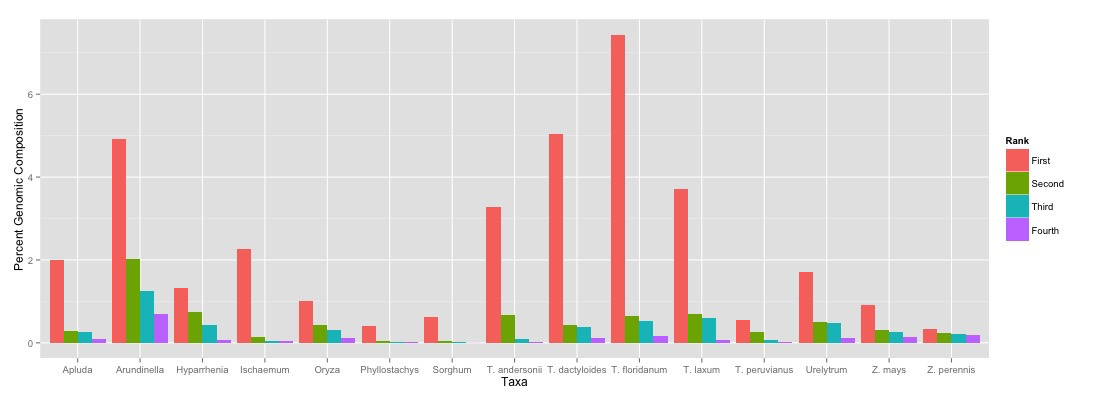
\includegraphics[width=4in]{Rankstrfcontent.png}
\end{center}
\caption{{\bf Genomic Composition of Top 4 Tandemly Repetitive Contigs .}
The top 4 contigs in each species were defined as not having homology to one another, in order to identify separate repeat motifs.
Species are ordered alphabetically by genus.
}
\label{ranktrf}
\end{figure}

\begin{figure}[h]
\begin{center}
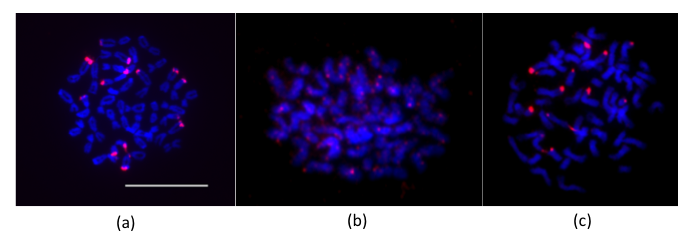
\includegraphics[width=4in]{FISH_Figure.png}
\end{center}
\caption{{\bf Fluorescent in-situ hybridization for the highest abundance tandem repeat monomer in for three grasses.}
(a) Arundinella, (b) Hyparhenia, (c) Urelytrum.
Not sure what other kind of text goes under FISH.}
\label{FISH}
\end{figure}

%\begin{figure}[h]
%\begin{center}
%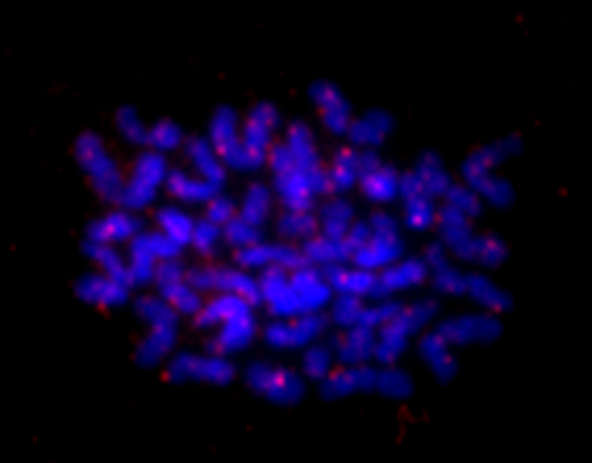
\includegraphics[width=4in]{Hypdip_TK177-Repet.png}
%\end{center}
%\caption{{\bf Fluorescent in-situ hybridization for the highest abundance tandem repeat monomer in Hypparhenia.}
%Still not sure what other kind of text goes under FISH.}
%\label{FISH2}
%\end{figure}
%
%\begin{figure}[h]
%\begin{center}
%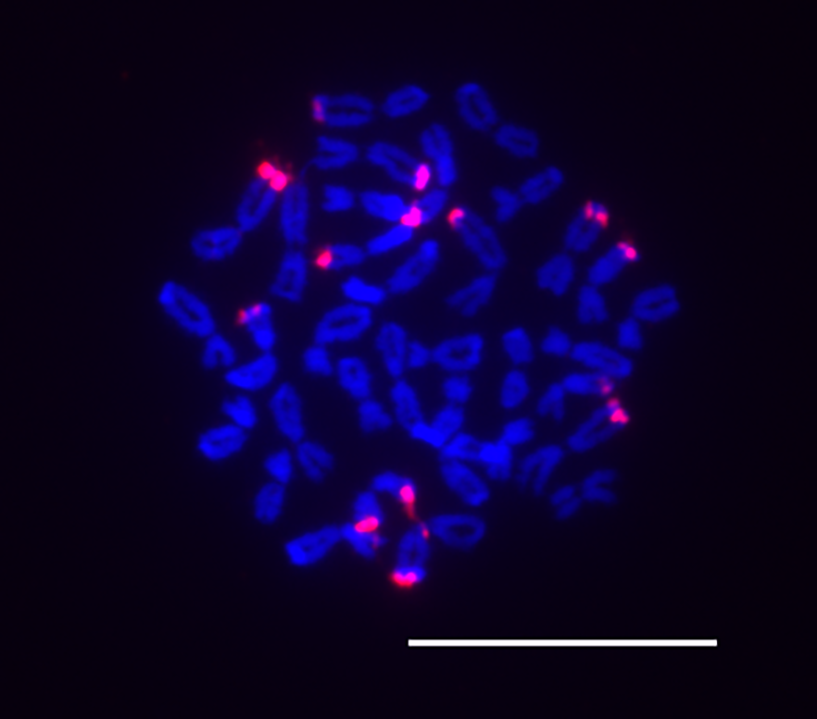
\includegraphics[width=4in]{Arundinella_19.png}
%\end{center}
%\caption{{\bf Fluorescent in-situ hybridization for the highest abundance tandem repeat monomer in Arundinella.}
%Still not sure what other kind of text goes under FISH.}
%\label{FISH3}
%\end{figure}

\section*{Discussion}

Our analyses of tandem repeats in grasses provides insight into the evolution of genome organization.
Most importantly, we show that previous assumptions about repeat abundance and function do not hold within all taxa examined in this study.
Genomic abundance was not predictive of centromere localization within the three novel repeats that were examined through FISH.
In \emph{Urelytrum} and \emph{Hyparrhenia}, FISH results did not suggest that the highest ranked contig was centromeric, as probe illumination was scattered across chromosomes, not often found near central locations, or confined to only some of the chromosomes (Figure \ref{FISH}).
While the \emph{Arundinella} probed repeat was also not centromeric, we believe that our de novo assembly and FISH has successfully identified another case of heterochromatic knob repeats.
The \emph{Ischaemum} repeat, which was not probed, shared short regions of homology with \emph{Sorghum}.
The \emph{Zea} and \emph{Tripsacum} repeats shared homology between many of their highest abundance tandem repeats, the highest abundance tandem repeat was homologous to a known repeat, indicative of the presence of knobs and CentC within both genera.
\emph{Sorghum}'s and \emph{Apluda}'s highest abundance repeat shared homology and sequence length. 
\emph{Phyllostachys} and \emph{Oryza}, although they were unique amongst our samples, shared homology with previously annotated bamboo and rice repeats.
Given the inconsistency of abundance as a predictor of centromere localization, we believe the method of chromatin immunopercipitation with cenh3 proteins (ChiP) published in Zhang et al \cite{zhang2014boom} can most reliably identify centromere repeats.
Our results show both rapid turnover and occasional retention of high abundance tandem repeats across our taxanomic sampling as well as a wide variance of tandem repeat abundance across grasses.

%Knobs are very unique genomic features, known to induce meiotic drive in maize \cite{}, suppress recombination locally but increase recombination between itself and the centromere \cite{}, and have only been identified in 2 other cases \cite{RYE??}.
%That we find no sequence homology between \emph{Arundinella} knobs and \emph{Zea} knobs suggests that we have identified the existence of an entirely novel knob.
%Interesting, the lengths of the knob variants between \emph{Arundinella} and \emph{Zea} are similar, centered around 180bp and 360bp.

%need to make sure this paragraph has the spin that de novo assembly and genome comp gives us a high throughput way of looking at tandem repeat evolution across many populations / species.  Not sure it does this enough.
De novo assembly of tandem repeats is an efficient, low cost opportunity to explore repetitive content in non-model genomes, an area of study generally left untouched due to the difficulties of traditional assembly.
In the assembly of the \emph{Arundinella} repeats, we show an example of how de novo assembly of tandem repeats can add to evolutionary biology.
\emph{Arundinella}, basal to all other species in this study, has two highly abundant tandem repeats that are unique over their full length that do not share large homology to any annotated genetic sequence.
Our cytological work suggests that these two sequences derive from knob-like heterochromatin.
Knobs are very unique genomic features, known to induce meiotic drive in maize \cite{dawe1996induction}, suppress recombination locally but increase recombination between itself and the centromere \cite{buckler1999meiotic}, and have only been identified in maize and rye\cite{gill1974giemsa}.
That we find no sequence homology between \emph{Arundinella} knobs and \emph{Zea} knobs suggests that we have identified the existence of an entirely novel knob.
Interestingly, the lengths of the knob variants between \emph{Arundinella} and \emph{Zea} are similar, centered around 180bp and 360bp.
Further work will be necessary to identify whether similar function concerning recombination and meiotic drive apply to the knobs of \emph{Arundinella}, but their existence suggests that knobs may be a more common evolutionary phenomenon than previously thought.
It is possible that such knob-like features eventually do result in the creation of novel centromeric sequences, offering an explanation that bridges the gap from an old centromeric repeat variant to a drastically different novel variant.
The ability to look broadly across a phylogeny at consensus repeats may provide a glimpse into the ancestral condition of tandem repeats of andropogonaeae; tandem repeats that may have become the structurally important but diverged centromere repeats of maize and sorghum.
The identification of novel repeats in previously unstudied organisms has the potential to produce phylogentically relevant data, shedding light on the evolution of the repetitive fraction of the genome.
Using consensus tandem repeats, evolutionary biologists can begin to piece together sequence turnover in repetitive regions \cite{henikoff2001centromere} and inform the ways in which these heterochromatic regions of the genome evolve.

The methods presented here can also be applied to study variation in genomic composition within and between species.
Genome size is highly variable across plants \cite{kewc} and is implicated with many important phenotypic traits such as flowering time and seed size \cite{rayburn1994selection,knight2005large}.
The ability to identify the percentage of the genome composed by specific types of tandem repeats can enable studies that track the components driving genome size variation.
When applied across populations of a species, researchers can test whether repetitive components that drive genome size change are under selection.
Looking across species, repetitive composition can inform our understanding of speciation, providing data toward the ideas of centromere repeat turnover and how frequently it coincides with speciation.
Also, identification of genomes with high abundance of tandem repeats may lead to a better understanding of selfish genetic elements and how they may influence long term evolution.
Two questions arise from our observations of genomic composition if the repetitive elements in \emph{Arundinella} are truly similar in their selfish function to the knob repeats in \emph{Tripsacum} and \emph{Zea}; what about the 180bp and 360bp repeat length allows them to expand to >5\% of the genome in grasses and why is there no sequence homology between the selfish repeats?\pb{yeah, its a semi colon, feels rocky but the point is important i think.  thoughts on better integration?}
Altogether, the results presented here show how de novo assembly can be used to better understand the repetitive fraction of the genome.

%Section 1: TRF/abundance as a way to identify de novo cent repeats (FAIL)
%Section 2: Other applications: can ID novel big repeats in nonmodel systems
%Section 3: Discuss genomic comp in our taxa, say we can see this method used to ID variation in genomic comp across a genus or populations, a way to start quantifying and documenting variation in repeat regions


%
%\subsection*{S2 Fig}
%\label{S2_Fig}
%{\bf Lorem Ipsum.} Maecenas convallis mauris sit amet sem ultrices gravida. Etiam eget sapien nibh. Sed ac ipsum eget enim egestas ullamcorper nec euismod ligula. Curabitur fringilla pulvinar lectus consectetur pellentesque.
%
%\subsection*{S1 Table}
%\label{S1_Table}
%{\bf Lorem Ipsum.} Maecenas convallis mauris sit amet sem ultrices gravida. Etiam eget sapien nibh. Sed ac ipsum eget enim egestas ullamcorper nec euismod ligula. Curabitur fringilla pulvinar lectus consectetur pellentesque.

\section*{Acknowledgments}
\nolinenumbers

%\section*{References}
% Either type in your references using
% \begin{thebibliography}{}
% \bibitem{}
% Text
% \end{thebibliography}
%
% OR
%
% Compile your BiBTeX database using our plos2015.bst
% style file and paste the contents of your .bbl file
% here.
% 
\bibliography{refdenovocent.bib}



\end{document}

